\chapter{Study and Results}
In this chapter we will present the study that has been performed and the results
generated using our simulation.

\section{The personality traits of children with ADHD}
A recent study \cite{Polanczyk2015} show that the world wide prevalence
for anxiety disorders within children and adolescents to be around 6.5\%, and 
Attention-deficit hyperactivity disorder (ADHD)\cite{Barkley1997} being one
of the most common childhood behavioral disorder, ranging between 5\% and 10\% \cite{Sayal2018}.

\bb

Because of the high prevalence of anxiety disorders in the general population,
and the availability of studies correlating ADHD with personality traits, we
decided to study the effect of children with personality profiles that match those
of ADHD patients on the class as a whole.

\bb

The primary reference for how ADHD symptoms relate to personality traits, we took
from \cite{Nigg2002}, where the authors write

\textit{\dots our findings for the two major symptom domains suggest the following
conclusion: overall ADHD symptoms are related to low Conscientiousness, low Agreeableness, and high Neuroticism.}

\section{Study Objective}
The study we performed had the objective to simulate how an increasing number of
students with ADHD symptoms would effect the group dynamics. This was achieved by
the following steps.

\begin{itemize}
    \item We defined three types of students (\textit{ADHD, Normal, Ambitious})
    \item Created several classroom profiles varying the ratio of the different student types present
    \item Run a Simulation study comparing the classroom profiles to each other
\end{itemize}

\subsection{Student Types}
The student types chosen have been in spired by the literature, whereby we 
took defined a ADHD student using results from \cite{Nigg2002}, a normal type using
\cite{Srivastava2003} and Ambitious students from \cite{Asendorpf2003}.

The concrete personality profiles used for each type are found in table \ref{StudenTypesTable}

\begin{table}[h!]
    \centering
    \begin{tabular}{|l|c|c|c|c|c|} 
        \hline
        \textbf{Student Type} & \textbf{O} & \textbf{C} & \textbf{E} & \textbf{A} & \textbf{N} \\
        \hline
        \hline
        ADHD & RND & 0.20 & RND & 0.20 & 0.80 \\
        \hline
        Normal & 0.75 & 0.60 & 0.55 & 0.65 & 0.50 \\
        \hline
        Ambitious & 0.80 & 0.80 & RND & 0.80 & 0.20 \\
        \hline
        Random & RND & RND & RND & RND & RND \\
        \hline
    \end{tabular}
    \caption{Table with Student types composition groups}
    \small RND indicates a random value from a uniform distribution between [0, 1]
    \label{StudenTypesTable}
\end{table}

\subsection{Groups}
Based on the student types we created various classrooms that where compared to
each other. Each group consisted of 30 students, varying the \% of each Student
type per group (see table \ref{GroupTable}).

\begin{table}[h!]
    \centering
    \begin{tabular}{|l|c|c|c|c|} 
        \hline
        \textbf{Group} & \textbf{ADHD} & \textbf{Normal} & \textbf{Ambitious} &  \textbf{Rabdom} \\
        \hline
        \hline
        ADHD-Low & 7\% & 93\% & 0\% & 0\% \\
        \hline
        ADHD-Medium & 17\% & 83\% & 0\% & 0\% \\
        \hline
        ADHD-High & 33\% & 66\% & 0\% & 0\% \\
        \hline
        ADHD-VeryHigh & 50\% & 50\% & 0\% & 0\% \\
        \hline
        ADHD-None & 0\% & 100\% & 0\% & 0\% \\
        \hline
        ADHD-Medium-Ambitious & 20\% & 40\% & 40\% & 0\%\\
        \hline
        ADHD-None-Ambitious & 0\% & 50\% & 50\% & 0\% \\
        \hline
        Random & 0\% & 0\% & 0\% & 100\% \\
        \hline
    \end{tabular}
    \caption{Groups composition studied}
    \small RND indicates a random value from a uniform distribution between [0, 1]
    \label{GroupTable}
\end{table}

\section{Results}
We have been simulation each of the groups defined above in 10 instances, meaning 
the same classroom configuration was simulation using 10 different seed values.

The HA-Plot generated by the last step of the Data Analysis is shown in figure \ref{StudyResults}.

\begin{figure}[]
    \makebox[\textwidth][l]{%
    \begin{minipage}[t]{500pt}
        \centering
        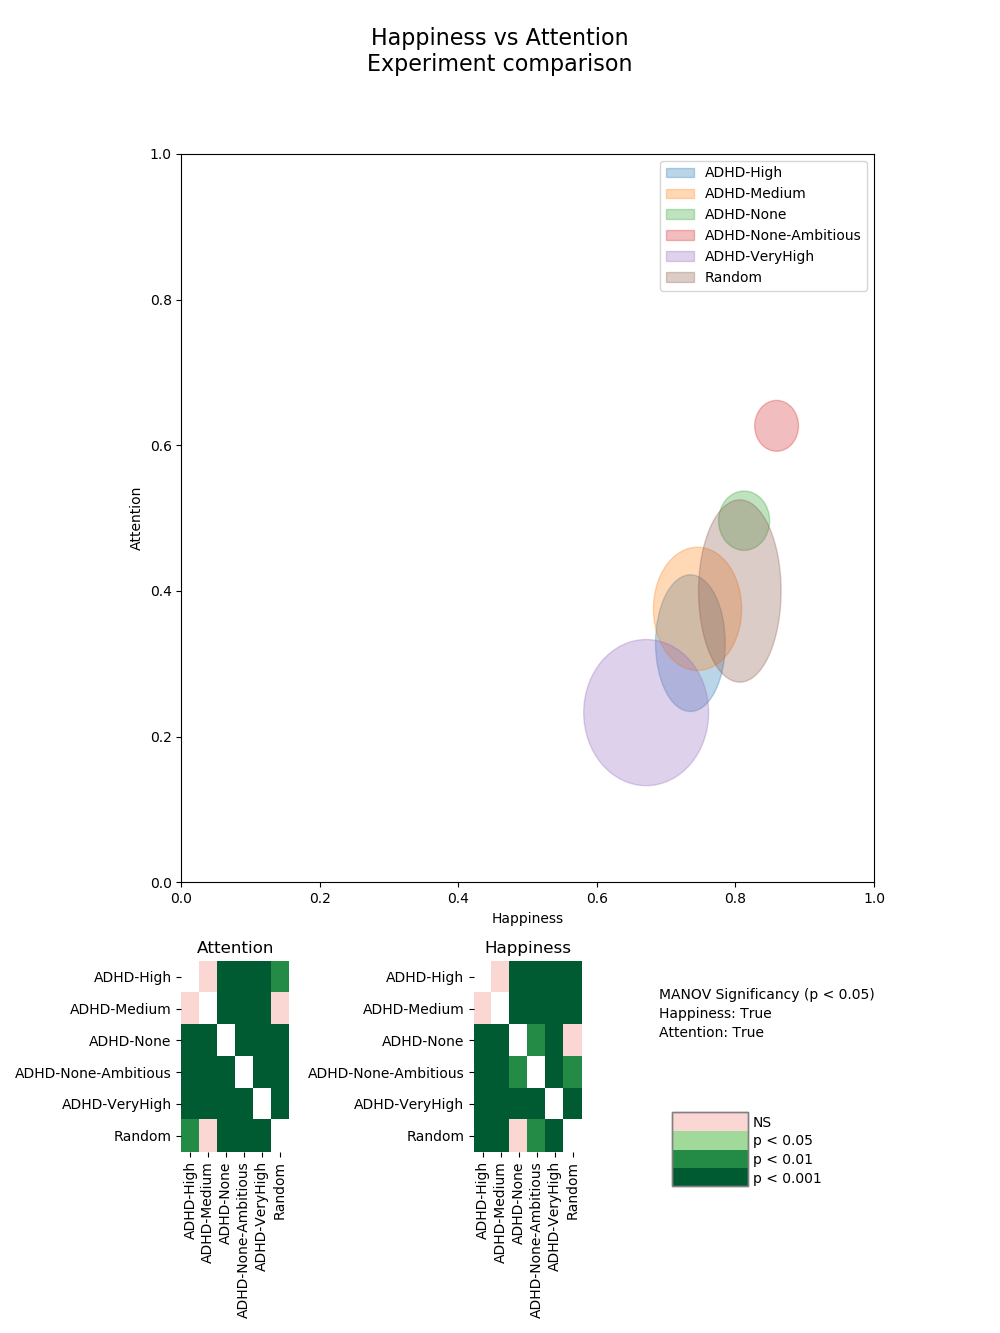
\includegraphics[width=400pt]{results/HAPlot}
        \caption{HA-Plot comparing the different classroom configurations}
        \label{StudyResults}
    \end{minipage}    
    }%
\end{figure}

\section{Discussion and Interpretation of Results}
Check some of the following properties

* Discuss HA-Plot averages, as well as difference in STD per group.

* How do the concrete Classroom aggregate plots differ?
    ** For example are there very repetitive patterns? Are there distortions in the pattern?
    ** Do any of the groups have stronger tendency to have more or less periods of intensive quarreling?

\dots


